\documentclass[a4paper,twocolumn]{article}
\usepackage{graphicx}
\usepackage{booktabs}
\usepackage{geometry}
\usepackage{fancyhdr}
\usepackage[skip=2pt]{caption}
\usepackage{indentfirst} 
\usepackage{titling}

% Adjust the margins to use the full space of A4 paper
\geometry{
  a4paper,
  left=17.018mm,
  right=17.018mm,
  top=20.066mm,
  bottom=12.954mm
}

\DeclareCaptionFormat{custom}
{%
    \scriptsize #1 \scriptsize #3
}
\captionsetup{format=custom}


% Set up the header and footer
\fancypagestyle{plain}{
  \fancyhf{}
  \fancyhead[L]{[FM23201]} % Left header
  \fancyfoot[R]{Supervisor[Prof.Makio Ishihara]} % Center footer
  \renewcommand{\headrulewidth}{0pt} % Remove header line
  \renewcommand{\footrulewidth}{0pt} % Remove footer line
}



\pagestyle{plain}
\setlength{\droptitle}{-4em}     % Eliminate the default vertical space
\addtolength{\droptitle}{-2pt}   % Only a guess. Use this for adjustment
\title{\textbf{The Development of Haptic Feedback Data Glove for Enhancing Immersion in VR Experiences}}
\author{\small{Korntawat Witchuvanit (Computer Science and Engineering)}}
\date{\vspace{-3em}}

\begin{document}
\small
\maketitle

% Redefine the section command to use a smaller font size and reduce spacing
\makeatletter
\renewcommand\section{\@startsection{section}{1}{\z@}%
  {-1.0ex \@plus -0.5ex \@minus -.2ex}%  % Adjust the spacing before the section title
  {0.3ex \@plus 0.2ex}%  % Adjust the spacing after the section title
  {\normalfont\small\bfseries}}
\makeatother



\section{Introduction}
Virtual reality (VR) provides immersive experiences through multisensory feedback, enhancing user interaction with digital environments. One key aspect of immersion is texture rendering, which is commonly achieved through visual and auditory cues. Incorporating haptic feedback for realistic texture perception is a mainstream of HCI research activities and it still remains a challenge. Most existing methods rely on hand-held devices, often limiting natural hand movements. This research explores the development and performance of a wearable device equipped with flex sensors, a Motion Processing Unit (MPU), and a coin motor, enabling texture perception at three vibration granularities.

\section{Related Work}
Deep-Texture [1] renders shapes and textures of things in VR using a linear resonant actuator and a 1-bar mechanism, employing three frequencies for texture simulation. A follow-up study [2] examines how vibrotactile parameters (granularity, amplitude, timbre) affect texture perception by synchronizing vibrations with user movement, finding that granularity influences the perception of bumpiness or smoothness. This research develops a data glove leveraging Pulse Width Modulation (PWM) to modulate granularity for texture rendering and discusses the feasibility of PWM. PWM has the advantage of high tolerance for noise from frequent movement of wires that connect sensors and motors.

\section{Haptic Feedback Data Glove}
The proposed device is a sensor-equipped glove designed to enable finger tracking while delivering realistic haptic feedback. The glove integrates multiple key components to enhance interaction and immersion. Flex sensors are attached to each finger, allowing the system to detect bending and movement, accurately measuring the degree of flexion to interpret finger gestures in real time. An MPU is embedded to track hand orientation, acceleration, and rotation, and it enables motion capture and seamless interaction within virtual environments. Micro-vibration motors are placed within the glove to enhance tactile realism and provide haptic feedback, generating subtle vibrations that simulate textures during virtual interactions.

\section{Experimental Setup}
Six male participants with the ages of 24 to 27 took part in a series of experiment to evaluate haptic feedback perception. The haptic feedback were generated using PWM at three different cycle rates: 0.2, 0.5, and 1.0, each representing a distinct texture sensation.\par
In the first experiment, participants conducted a blind test to distinguish between three different haptic feedback. Before starting, they were introduced to all three haptic feedback. A white 3D plane then appeared in the virtual environment, randomly generating one of the feedback upon contact with the virtual hand. The participants identified the perceived feedback, repeating the process 15 times to assess their ability to differentiate between them.\par
The second experiment explored the relationship between haptic feedback and texture perception. The participants interacted with a textured 3D plane with  three different granularities of brick, grass, or marble, each generating three different haptic feedback. After experiencing all three feedback for a given texture, they were asked to select the one they felt best matched the material before proceeding to the next texture.\par
They completed an evaluation questionnaire after the experiments. 					

\section{Results}
The results indicate that in the blind test involving three haptic feedback, the  participants were able to distinguish between the lowest cycle rate (0.2) and the highest one (1.0), as shown in Fig. 1. However, the scores for the middle one (0.5) were similar to those of the lowest one. Some participants noted that the glove is too big for my hand, making it difficult to identify the granularities accurately. This may be due to the use of a standard glove with an attached component, which cannot be adjusted to fit every hand.\par
The result from the second experiment is shown in Fig.2. The marble which represents the smoothest material is compatible with 1.0 cycle rate while the grass is likely to go with 0.5 cycle rate and the last one that represents the least smoothness is equally for 0.2 and 0.5 cycle rate.

\begin{figure}[h]
  \centering
  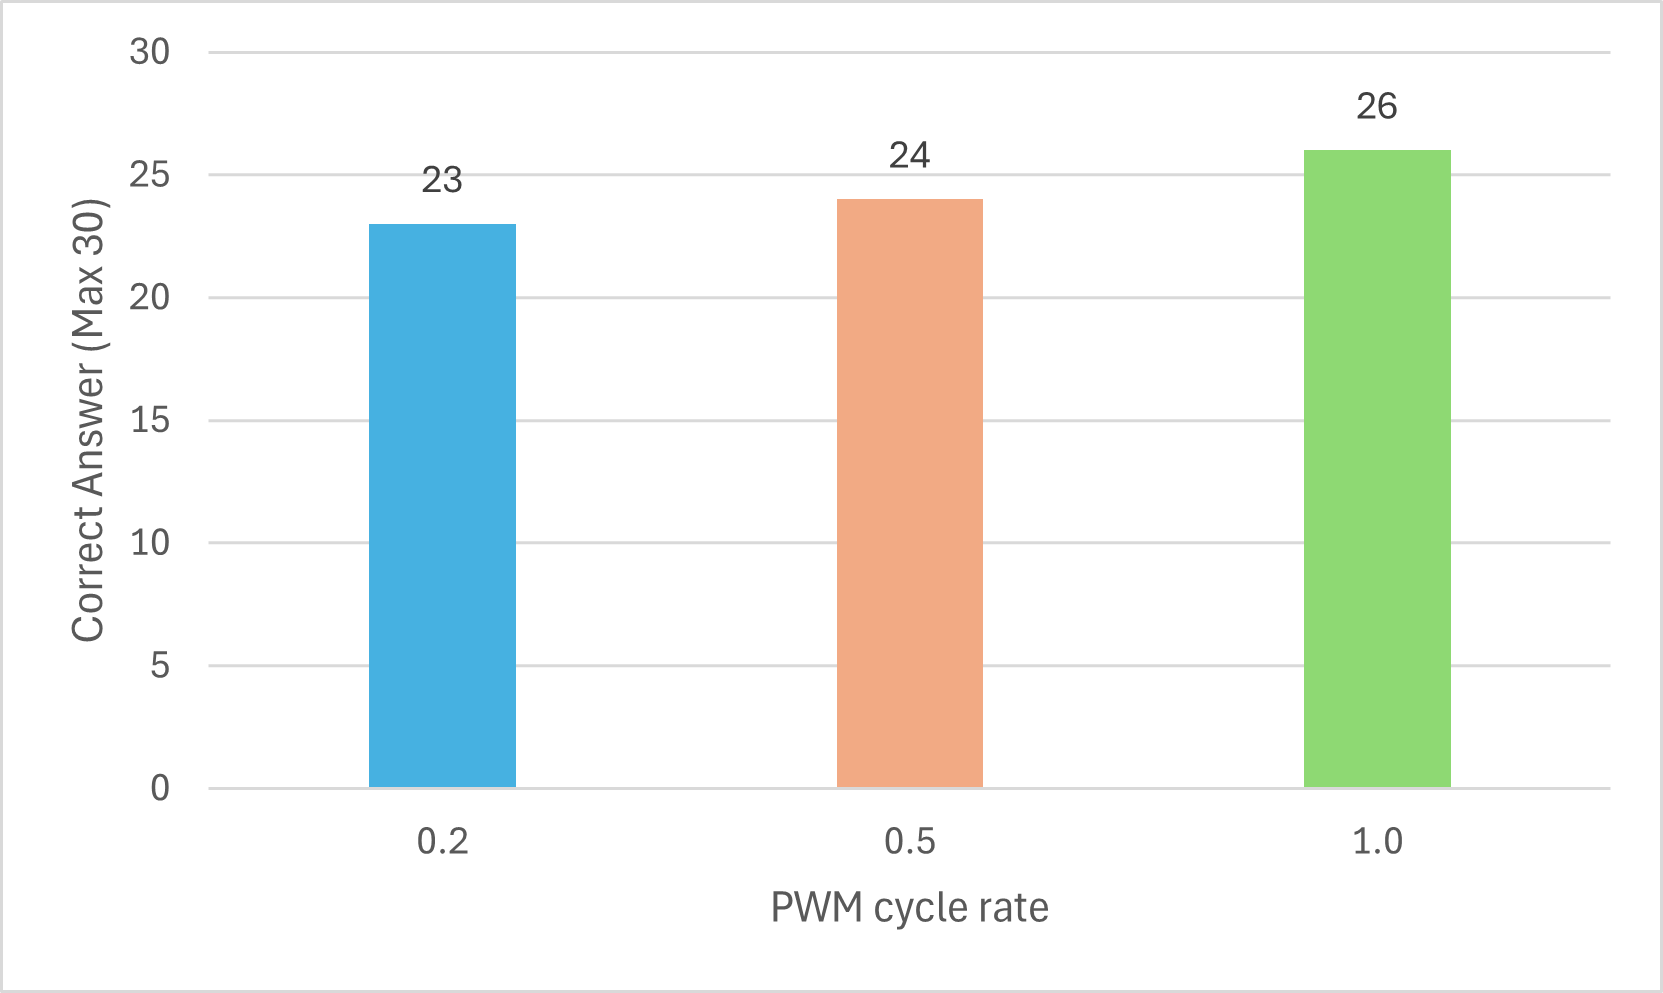
\includegraphics[width=0.35\textwidth]{./Fig/PWM_Correct_Test.png}
  \caption{{Result of First Experiment}}
  \label{fig1}
  \vspace{0.1cm}
  \centering
  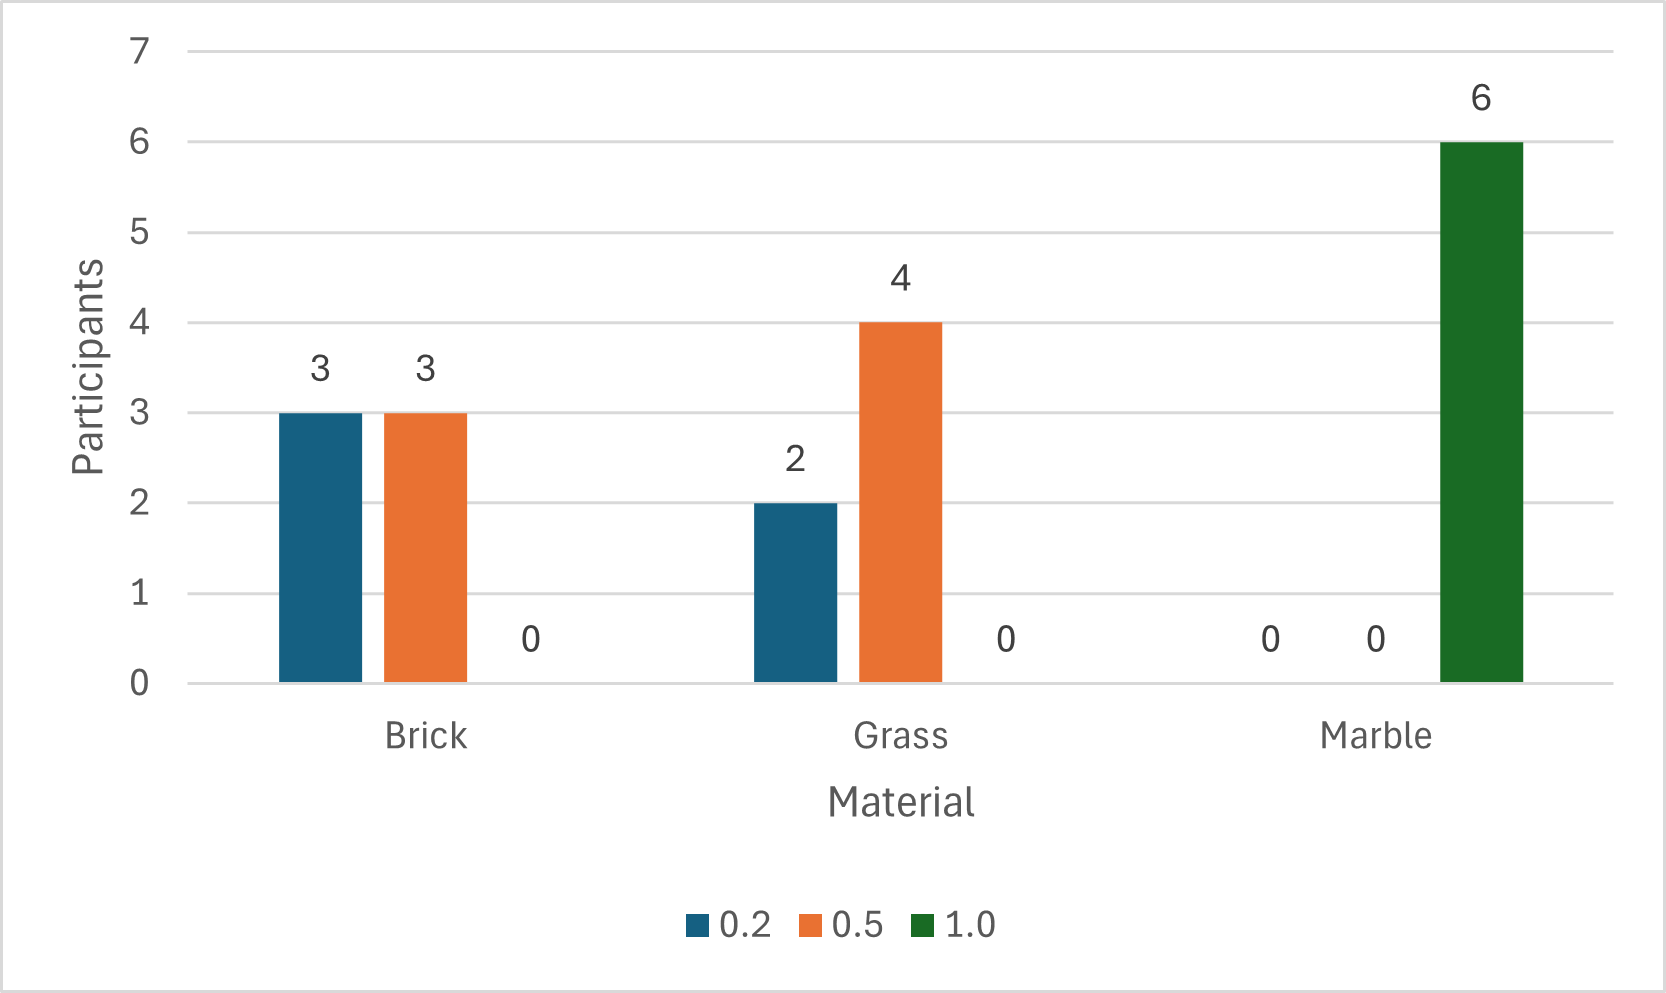
\includegraphics[width=0.35\textwidth]{./Fig/Texture_Select_Test.png}
  \caption{{Result of Second Experiment}}
  \label{fig2}
\end{figure}


\section{Conclusion}
The results show that participants could distinguish between the lowest cycle rate (0.2 )and highest one (1.0) of haptic. Additionally, material smoothness influenced preferred cycle rate, with marble aligning with 1.0 cycle rate, grass with 0.5 cycle rate. These findings highlight the feasibility of PWM for haptic rendering of textures.

\begin{thebibliography}{99}
  \scriptsize
    \bibitem{sdn1} Y. Sung, D. Kwak, T. Kim, W. Woo and S. H. Yoon, "Deep-Texture: A Lightweight Wearable Ring for Shape and Texture Rendering in Virtual Reality," 2024 IEEE Conference on Virtual Reality and 3D User Interfaces Abstracts and Workshops (VRW), Orlando, FL, USA, 2024, pp. 911-912
    \bibitem{sdn2} Paul Strohmeier and Kasper Hornbæk. 2017. Generating Haptic Textures with a Vibrotactile Actuator. In Proceedings of the 2017 CHI Conference on Human Factors in Computing Systems (CHI '17). Association for Computing Machinery, New York, NY, USA, 4994–5005.
\end{thebibliography}

\end{document}


% Ref. for Figures and Tables
% \begin{table}[ht]
%     \centering
%     \begin{tabular}{|c|c|c|}
%         \hline
%         Condition & Score & Comment \\
%         \hline
%         A & 5.0 & Good \\
%         B & 3.8 & Average \\
%         C & 2.5 & Poor \\
%         \hline
%     \end{tabular}
%     \caption{Experimental Results}
%     \label{tab:results}
% \end{table}

% \begin{figure}[ht]
%     \centering
%     \includegraphics[width=0.8\linewidth]{example-image} % Replace with your figure
%     \caption{Experimental Result 1}
%     \label{fig:result1}
% \end{figure}